\documentclass[preprint,showpacs,nofootinbib,floatfix]{revtex4-1} 
\usepackage{graphicx}
\usepackage{amssymb}
\usepackage{amsmath}
\usepackage{amsthm}
\usepackage{amsfonts}

\begin{document}

Just a simple \LaTeX\ file.

Now, let's add something!

\end{document}



\vspace*{-5pt}
\begin{figure}[h!]
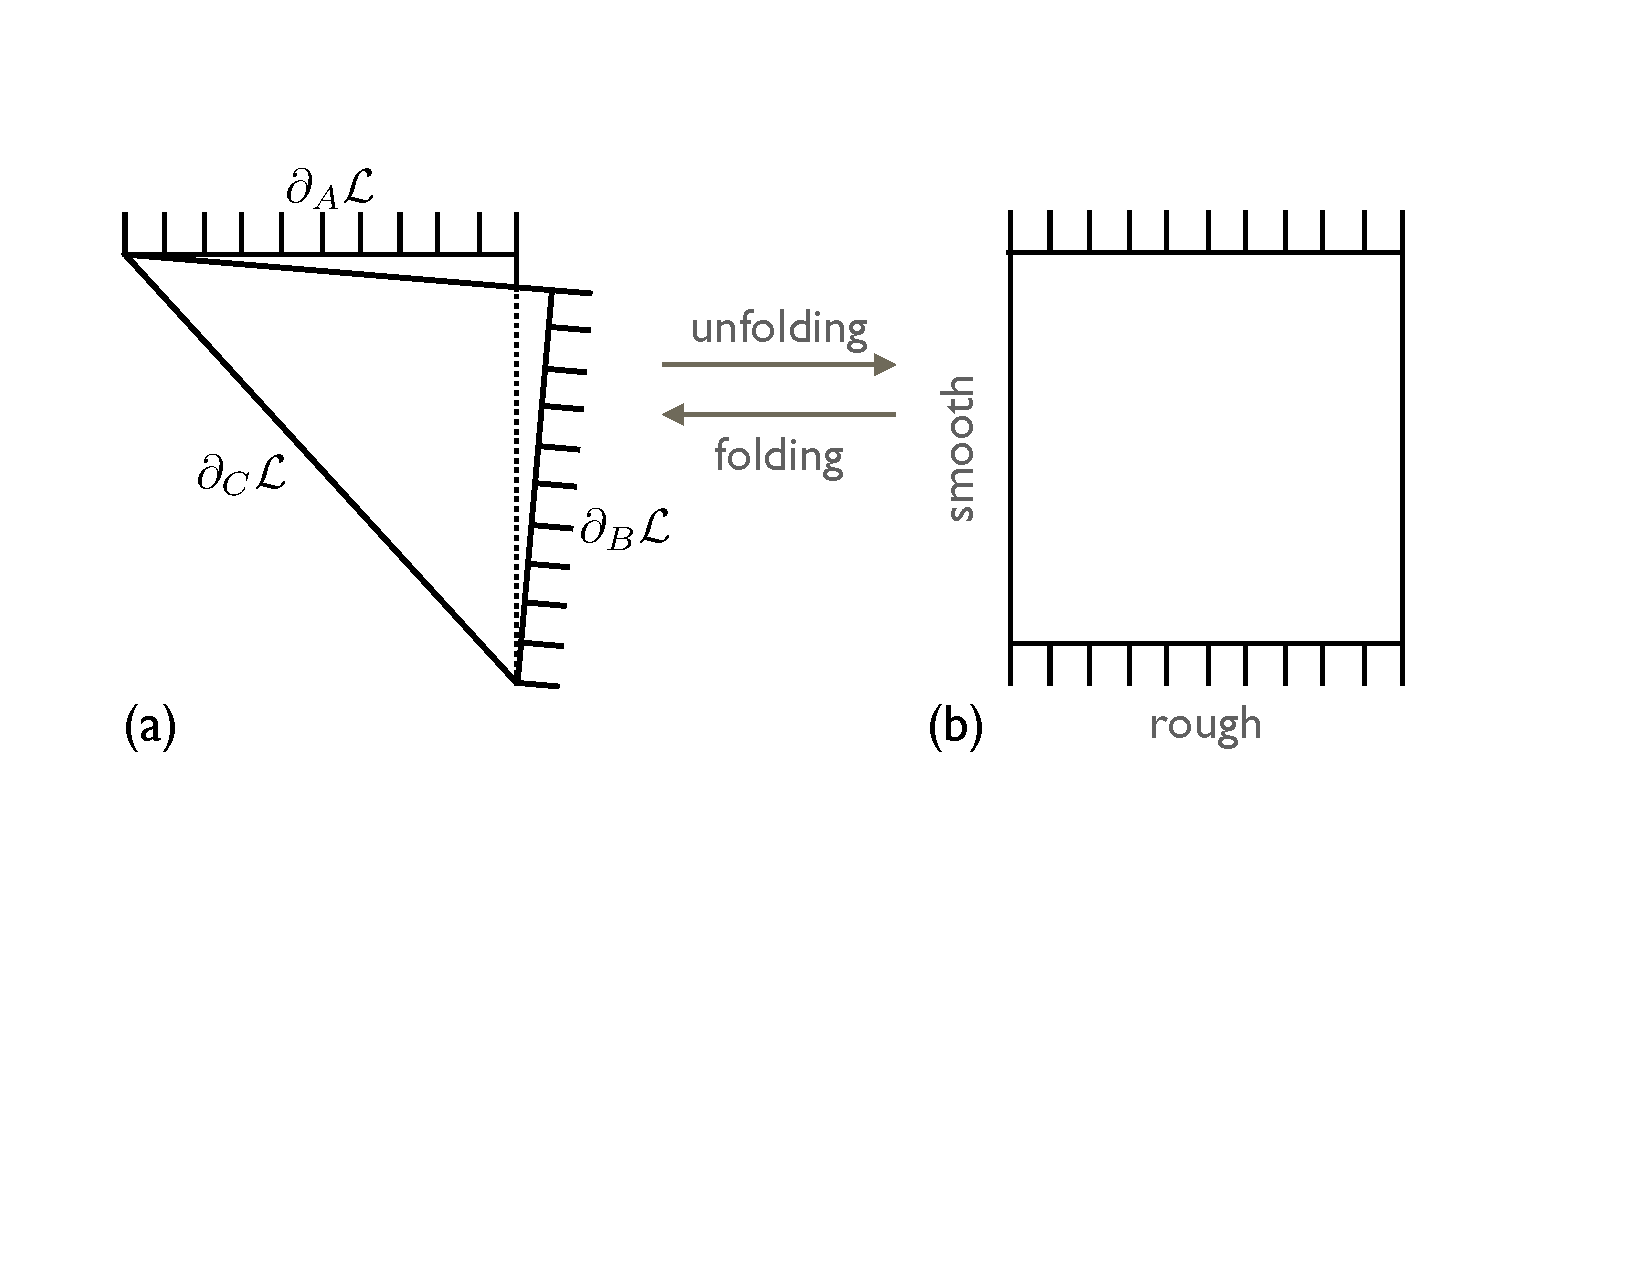
\includegraphics[width=0.70\textwidth]{fig_fold2}
\vspace*{-5pt}
\caption{The topological color code (a) with three boundaries $\partial\mathcal{L}^A$, $\partial\mathcal{L}^B$ and $\partial\mathcal{L}^C$ viewed as the folded toric code (b) with two smooth and two rough boundaries. The boundary $\partial\mathcal{L}^A$ of color $A$ is equivalent to a pair of boundaries --- smooth in the front and rough in the rear layer; similarly $\partial\mathcal{L}^B$. The boundary $\partial\mathcal{L}^C$ is the fold.}
\label{fig_folding} 
\end{figure} 
